\documentclass[compress]{beamer}
\usepackage{graphics}
\usepackage{hyperref}
\hypersetup{
    colorlinks,
    citecolor=blue,
    filecolor=black,
    linkcolor=blue,
    urlcolor=blue,
    bookmarksopen = false,
    %pdfstartview = {XYZ null null 1.00}
 	%pdfpagemode=None
}
\usepackage{amsmath}
\usepackage{beamerthemesplit}
\usepackage{multicol}
\usetheme[hoptionsi]{Madrid}
%\usetheme{CambridgeUS}
\useinnertheme{rectangles}
%\usecolortheme{dolphin}
 \title[Masters Dissertation]{Masters Dissertation}
 \subtitle {``Smart Cafeteria'' Adaptive And Interactive Mobile Application}
 \logo{%
    
\includegraphics[width=1cm,height=1cm,keepaspectratio]{Logo/logo}~%
}
%\author[Supta R. Philip] % (optional, use only with lots of authors)
%{\textbf{Supta Richard Philip}~\inst{1}}
\author[Supta R. Philip]{\textbf{Supta Richard Philip}~\inst{1}\\{\small{Supervisor: Professor Antonella De Angeli}}}
% - Give the names in the same order as the appear in the paper.
% - Use the \inst{?} command only if the authors have different
%   affiliation.
\institute[University of Trento] % (optional, but mostly needed)
{
  \inst{1}%
  M.Sc. in Computer Science\\
  Department of Information Engineering
and Computer Science\\
  University of Trento, Italy.
  \\[\medskipamount]
     % 
\includegraphics[width=\textwidth,height=.5\textheight]{Logo/logo}%
      
\includegraphics[width=2.5cm,height=2.5cm]{Logo/logo}%
  %\\\scalebox{2}{\insertlogo}
  
  }
  
  
 \date [\today]{\today
%  \\ \ \\
%  \tiny{ Copywrite Declaration : Metarials are taken from Dr. Ashfaqur Rahman, Research Scientist,Intelligent Sensing and Systems Lab (ISSL),CSIRO, Australia \& \\
% Xiaohua Jia, Chair Professor,Dept of Computer Science,City University of Hong Kong.}
%  
 }

\AtBeginSection[]{
%   \setbeamercolor{section in toc shaded}{use=structure,fg=structure.fg}
%   \setbeamercolor{section in toc}{fg=mycolor}
%   \setbeamercolor{subsection in toc shaded}{fg=black}
%   \setbeamercolor{subsection in toc}{fg=mycolor}
  \frame<beamer>{\begin{multicols}{2}
  \frametitle{Outline}
  \setcounter{tocdepth}{2}  
  \tableofcontents[currentsection,subsections]
\end{multicols} 
 }
}

 \begin{document}
 
 {
 	 \begingroup
	\addtocounter{framenumber}{-1}
 	 %gets rid of bottom navigation bars
	\setbeamertemplate{footline}{}
	\setbeamertemplate{logo}{}
	%gets rid of navigation symbols
	\setbeamertemplate{navigation symbols}{}
 	\frame{
 	\addtocounter{framenumber}{0}
 	\titlepage
 	}
 	\endgroup
}

 \section*{Outline}
 \phantomsection
%\addcontentsline{toc}{sec}{Outline}
 \frame<beamer>{\begin{multicols}{2}
  \frametitle{Outline of Thesis}
  \setcounter{tocdepth}{2}  
  \tableofcontents
\end{multicols} 
 }

\section[background]{Thesis Background}

\begin{frame}\frametitle{Thesis Background}
\textbf{``Smart Cafeteria''}
 \begin{itemize}
 \item is a part of Smart Campus Project. \\
  
\includegraphics[height=1.5cm,width=1.5cm]{images/smartcampuslab.png} \\
 \url{http://www.smartcampuslab.it/}


 \item Smart Campus has funded by Trento RISE. \\
 
\includegraphics[height=1.5cm,width=2cm]{images/trentorise.jpg} \\
 \url{http://www.trentorise.eu/}
 \end{itemize}
\end{frame}

\section[Statement]{Problem Statement}
\subsection{Scenarios}
\begin{frame}[allowframebreaks]\frametitle{Scenarios}

\begin{block}{Hungry Students}
  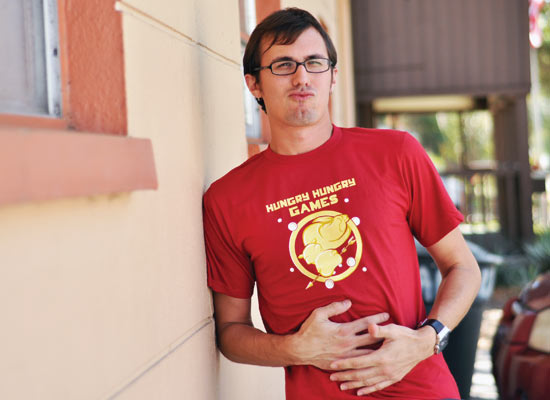
\includegraphics[height=4.5cm,width=4.5cm]{images/hungrystudent.jpg}
  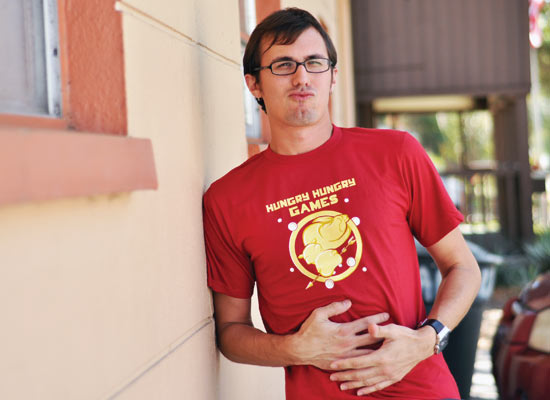
\includegraphics[height=4.5cm,width=4.5cm]{images/hungrystudent.jpg}
\end{block} 

\framebreak

\begin{block}{Busy Professors}
  
\includegraphics[height=1.5cm,width=1.5cm]{images/smartcampuslab.png}

\end{block} 

\end{frame}

\subsection{The Problem}
\begin{frame}[allowframebreaks]\frametitle{The Problem}
\begin{block}{Create ``Smart Cafeteria''}
Will be supported by:
\begin{itemize}
 \item web 2.0 Technologies.
 \item Smartphone application.
 \end{itemize}

\end{block}

\framebreak

\begin{block}{``Smart Cafeteria''}
application should be
\begin{itemize}
 \item Adaptive.
 \item Interactive.
 \end{itemize}
 \end{block}
\end{frame}

\section[Objective]{Objective}
\begin{frame}\frametitle{Objective}
\begin{block}{Proposed Services}
 \begin{itemize}
 \item  Mensa Queue Skipper.
 \item  Menu Finder.
 \item  Menu Suggester and Dieting Adviser.
 \item  Customized Menu creator.
 \item  Lunch with Friends.
 \end{itemize}
 \end{block}
\end{frame}


\section[Analysis]{Analysis}
\subsection{Stakeholders}
\begin{frame}\frametitle{Stakeholders}
\begin{block}{Stakeholders}
 \begin{itemize}
 \item  System Users.
 \begin{itemize}
 \item  Students.
 \item  Professors.
 \item  Researchers.
 \item  University�s Administration Officer.
 \item  University�s Technical Staff.
 \end{itemize}
 \item  System Administrator.
  \begin{itemize}
 \item  Cafeteria Staffs.
 \end{itemize}
 \end{itemize}
  \end{block}
\end{frame}

\subsection{Functional \& Non Functional Requirements}
\begin{frame}\frametitle{Functional \& Non Functional Requirements}
\begin{block}{Functional Requirements}
42 FR
\end{block}
\begin{block}{Non Functional Requirements}
Usability
Internationalization
Portability
Adaptability
\end{block}
\end{frame}

\subsection{Data Gathering \& More Requirements }
\begin{frame}\frametitle{Data Gathering \& More Requirements}
\begin{block}{Data Gathering \& More Requirements}
 \begin{itemize}
 \item  Studying Cafeteria�s Food Menu and Documents.
 \item  Focus Group - 7 participants.
 \item  Questionnaires.
 \end{itemize}
\end{block}
\begin{block}{Outcomes}
 \begin{itemize}
 \item  The application is usefull.
 \item  QR BARCODE.
  \item UML of application (Use case, Class Diagram, etc.)
 \end{itemize}
\end{block}
\end{frame}

\section[Design]{Design}
\subsection{Desktop Prototype}
\begin{frame}\frametitle{Desktop Prototype}

\end{frame}

\subsection{Mobile Prototype}
\begin{frame}\frametitle{Mobile Prototype}

\end{frame}

\subsection{Features of Smart Cafeteria}
\begin{frame}\frametitle{Features of Smart Cafeteria}

\end{frame}

\section[Evaluation]{Usability Evaluation}
\subsection{Evaluation Methodology}
\begin{frame}\frametitle{Evaluation Methodology}
User studies and questionnaire Methodology\\
Target Users (10) students\\
Given them 9 tasks to perform\\
Given them 14 questions to test (i) usefulness, (ii) easy to use, (iii) learnability and (iv) Satisfaction\\
Both Desktop and Mobile Prototype was evaluated.

\end{frame}

\subsection{Evaluation Result}
\begin{frame}\frametitle{Evaluation Result}
the result was analyzed calculating Mean($\mu$) and Standard deviation($\sigma$).

Standard Deviation, $\sigma$ =  $\sqrt{\frac{1}{N}\sum_{i}^{N} (x_i - \mu^2)} $
where Mean, $\mu$ = $\frac{1}{N}\sum_{i}^{N} x_i$.
\end{frame}

\begin{frame}\frametitle{Result for desktop Prototye}
Result for desktop

\end{frame}
\begin{frame}\frametitle{Result for Mobile Prototye}
Result for Mobile
\end{frame}

\section[Conclusion]{Conclusion}
\subsection{Future Work}
\begin{frame}\frametitle{Future Work}


\end{frame}

\subsection{Questions}
\begin{frame}\frametitle{Questions}
\begin{center}
\textbf{\textsc{Any Questions}} \\

\includegraphics[height=4cm,width=4cm]{images/question.jpg} \\
\textbf{Thanks}
\end{center}

\end{frame}

\end{document}